\documentclass[10pt,twocolumn,letterpaper]{article}
\usepackage[review]{cvpr}
\usepackage{graphicx}
\usepackage{booktabs}
\usepackage{amsmath,amssymb}
\usepackage{multirow}
\usepackage{xcolor}
\usepackage{url}
\usepackage{microtype}
\graphicspath{{figures/}}

\usepackage{placeins}
\definecolor{cvprblue}{rgb}{0.21,0.49,0.74}
\usepackage[pagebackref,breaklinks,colorlinks,allcolors=cvprblue]{hyperref}
\def\paperID{*****}
\def\confName{CVPR}
\def\confYear{2026}
\title{When Agreement Hides Error:\
Shared Measurement Influence in MRI Slice Interpolation}

\begin{document}
\maketitle

\begin{abstract}
Prediction disagreement is widely used as reliability evidence, yet it can be small when estimates share the same error. We study this failure in deterministic MRI inter-slice interpolation, where the physical measurements supporting a missing target can be controlled. Target-preserving measurement-disjoint contexts rank reconstruction error better than dependence-preserving controls on fastMRI, IXI, and NingXia: disjoint-minus-shared Spearman differences are .092, .095, and .193, with patient/examination-clustered confidence intervals above zero. Under clean sharing, 97.4--99.7\% of paired error energy is common to the two predictions. An exact analytical ladder rejects shared-anchor count as a sufficient monotone explanation. Instead, analytical coefficient influence and a local neural finite-response influence statistic predict error alignment and observable error fraction more strongly than overlap count. The neural advantage holds for HAT and SwinIR across all three broad context grids; an exact fixed-count test confirms it on fastMRI and 115-case IXI but is null/mixed in the eight-patient NingXia cohort. As a practical consequence, acquired-anchor cross-validation ranks examination-level interpolation difficulty ($\rho=.943/.955/.958$) and retrospective densification benefit, while remaining statistically similar to simple adjacent-anchor differences. The result is a mechanism and design principle, not calibrated uncertainty or a universally superior score: disagreement is informative only to the extent that its generating measurements exert sufficiently independent influence.
\end{abstract}

\section{Introduction}
Sparse through-plane MRI is routinely densified by interpolation or learned slice synthesis. A reconstruction can look anatomically plausible while smoothing, displacing, or inventing structure, so a reliability signal is desirable when dense targets are absent. Ensembles, test-time transformations, and cross-context consistency commonly use output variation as such a signal \cite{lakshminarayanan2017ensembles,gal2016dropout,edupuganti2021uncertainty}. Their appeal is intuitive: if plausible predictors disagree, at least one deserves scrutiny. Their blind spot is equally fundamental but less often controlled experimentally: predictors can agree because they reuse the same influential information and therefore make aligned errors.

We turn this abstract dependence problem into a physical intervention. For one missing MRI slice, phase-shifted acquisition grids can provide reconstruction contexts that preserve the target while changing which acquired slice anchors support it. This makes it possible to ask not merely whether outputs differ, but whether dependence among their generating measurements determines which target-error components disagreement can observe.

Figure~\ref{fig:mechanism} states the proposed chain. For predictions $f_a=y+e_a$ and $f_b=y+e_b$, output separation observes $e_a-e_b$. Shared measurements can induce similar local estimator responses; similar responses can align $e_a$ and $e_b$; aligned errors cancel in the difference. The elementary identity is not our novelty. The scientific question is what determines the error inner product. Our evidence identifies shared local measurement influence as one determinant in MRI interpolation.

This formulation also explains why a tempting early hypothesis failed. Integer anchor overlap has the right overall trend but is not a monotone dose: one weak shared anchor can matter less than another, and an exact four-anchor ladder reverses at zero-to-one overlap. We therefore replace count by estimator influence. For analytical interpolation this is derived from coefficients. For frozen HAT and SwinIR networks it is approximated by the cosine between output responses to identical finite perturbations of the same physical anchor. The quantity is explicitly local to a target, context, input, and plane.

Our contributions are threefold. First, we establish and decompose \emph{consensus blindness} with same-target, measurement-controlled interventions across three MRI cohorts and four estimator families. Second, we show that shared estimator influence explains error alignment and disagreement observability more strongly than raw overlap count, while retaining the NingXia fixed-count nonreplication and physical-plane dependence as boundaries. Third, we show a lightweight consequence: withholding acquired anchors yields an examination-level difficulty and retrospective densification-value signal without dense targets at scoring time, additional training, or repeated neural inference. It is useful but not uniquely superior to adjacent-anchor differences. The main result is thus a mechanism for when disagreement is trustworthy, rather than another uncertainty leaderboard.

\begin{figure*}[t]
\centering
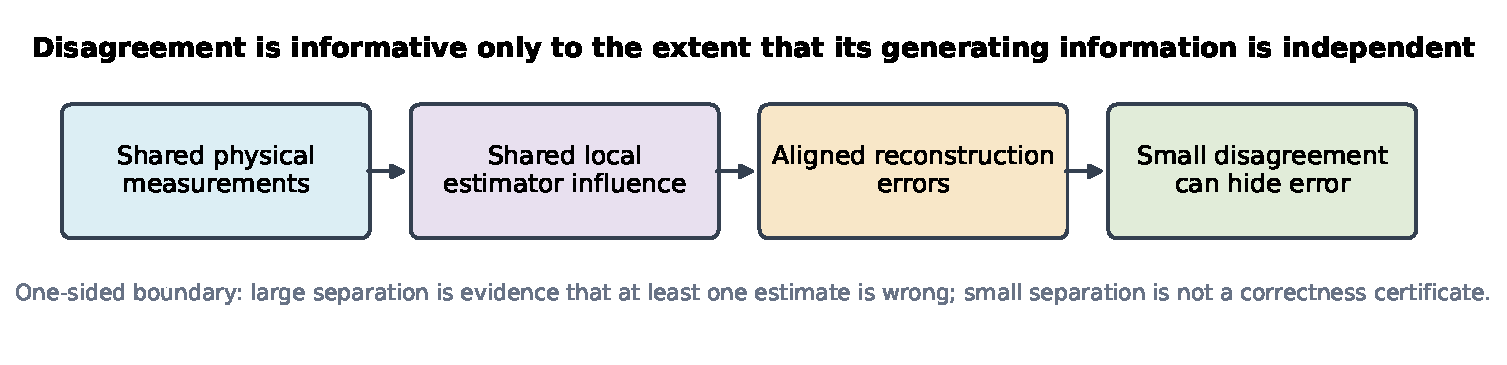
\includegraphics[width=.98\textwidth]{fig1_mechanism.pdf}
\caption{Proposed mechanism and reliability boundary. Reusing a physical measurement is not itself decisive; what matters is how similarly that measurement influences both local estimators. Aligned errors cancel in prediction differences. Large separation is one-sided evidence that at least one estimate is inaccurate, but small separation cannot certify correctness.}
\label{fig:mechanism}
\end{figure*}

\section{Related Work}
\paragraph{MRI reconstruction and uncertainty.}
Probabilistic, Bayesian, ensemble, and posterior-sampling methods quantify uncertainty in accelerated MRI \cite{edupuganti2021uncertainty,narnhofer2022bayesian,kustner2024ensembles,luo2023diffusion}. Training-free posterior approximation also addresses uncertainty in computational inverse problems \cite{zhang2024trainingfree}. These methods estimate predictive distributions or risk. Hu \etal showed that uncertainty variation can miss systematic MRI reconstruction error \cite{hu2021predict}. We study a narrower complementary question: how dependence between the physical measurements generating two deterministic predictions changes the target error visible in their disagreement.

\paragraph{Diversity, consistency, and dependence.}
Deep ensembles use predictive diversity for uncertainty \cite{lakshminarayanan2017ensembles}; diversity interacts with individual error and generalization rather than replacing them \cite{brown2005diversity,ortega2022diversity}. MRI self-consistency methods such as SPIRiT enforce compatibility with acquired measurements \cite{lustig2010spirit}. Our intervention differs from both: we hold the missing target fixed, explicitly manipulate reuse of physical slice measurements, and relate their estimator influence to target-error alignment and observability.

\paragraph{Slice synthesis and acquisition design.}
SAINT and I3Net learn anisotropic medical slice synthesis \cite{peng2020saint,song2024i3net}; single-stack slice-to-volume reconstruction couples interpolation and motion \cite{young2024svr}. Leave-one-slice-out interpolation checks predate this work \cite{horvath2017highorder}. Shifted multi-slice super-resolution and acquisition-design studies exploit complementary measurements for reconstruction accuracy \cite{greenspan2002interslice,nicastro2022shift}. We neither introduce a new interpolator nor claim the holdout operation as novel. Our distinction is using same-target physical dependence as a controlled variable for reliability observability.

\section{From Disagreement to Shared Influence}
\subsection{Error observability}
Let $y$ be the missing target slice and $f_i=y+e_i$ two deterministic reconstructions. Then
\begin{equation}
 \|f_a-f_b\|^2=\|e_a\|^2+\|e_b\|^2-2\langle e_a,e_b\rangle .
 \label{eq:difference}
\end{equation}
Writing $\bar e=(e_a+e_b)/2$ and $\delta=(e_a-e_b)/2$ gives
\begin{equation}
 \tfrac12(\|e_a\|^2+\|e_b\|^2)=\|\bar e\|^2+\|\delta\|^2 .
 \label{eq:decomp}
\end{equation}
We call the normalized terms \emph{shared} and \emph{observable} error fractions. If $e_a=e_b\neq0$, disagreement is zero despite error; if $e_a=-e_b$, all paired error energy is observable. Equation~\ref{eq:difference} is a starting identity. The mechanism question is what makes $\langle e_a,e_b\rangle$ large.

The same geometry gives a one-sided statement. By the triangle inequality,
\begin{equation}
 \max(\|e_a\|,\|e_b\|)\geq \tfrac12\|f_a-f_b\| .
 \label{eq:onesided}
\end{equation}
Large separation therefore certifies that at least one reconstruction has nonzero error of a corresponding scale. No converse exists: the right side can vanish for arbitrarily large common error. This asymmetry is why we use \emph{observability} rather than calibration terminology. Disagreement may supply evidence of failure, but agreement cannot by itself supply evidence of correctness.

\subsection{Analytical and neural influence}
For a local linear estimator $f=\sum_j c_jx_j$, embed two contexts in the union of physical anchor positions, with zero coefficients at unused anchors. Overlap count records common nonzero locations but ignores their unequal weights. We use coefficient cosine, signed dot product, and common absolute mass
\begin{equation}
 I_{\cap}(a,b)=\sum_j\min(|c_{a,j}|,|c_{b,j}|)
 \label{eq:mass}
\end{equation}
as analytical influence summaries.

For a frozen nonlinear interpolator $F_c$, we perturb the same shared physical anchor $j$ in contexts $a$ and $b$ with an identical seeded field $\epsilon\xi_{js}$. The centered output response is
\begin{equation}
 r_{cjs}=F_c(x+\epsilon\xi_{js})-F_c(x).
\end{equation}
Neural shared influence is the mean response cosine between $r_{ajs}$ and $r_{bjs}$ over shared anchors and four frozen seeds. The primary perturbation is a centered Rademacher field at 1\% of the globally normalized case range. This is a local response approximation, not a global coefficient, attribution theorem, or property of a network independent of target and plane.

\section{Experimental Design}
\subsection{Cohorts and frozen estimators}
We use 24 held-out fastMRI brain T2 examinations \cite{knoll2020fastmri}, 115 held-out IXI brain T2 examinations \cite{ixi_dataset}, and 22 out-of-fold NingXia knee T2 series from eight patients. NingXia inference resamples patients with all subordinate series retained. Frozen HAT and SwinIR $\times4$ reconstructions test nonlinear influence; linear and cubic interpolation provide analytical cross-estimator support. fastMRI and IXI also support the frozen retrospective $\times4\!\rightarrow\!\times2$ consequence. Dense slices create retrospective anchors and evaluate errors but never enter a reliability score. All primary scores reduce to one value per examination before cohort analysis.

\subsection{Controlled measurement contexts}
The zero-overlap condition reconstructs the same missing plane from phase-0 and phase-2 $\times4$ lattices. A clean maximal-sharing control applies horizontal flip equivariance to identical anchors while preserving target, anchor identity, $z$ order, distances, count, mask, and preprocessing. The primary endpoint is the Spearman correlation between masked prediction disagreement and paired reconstruction MAE. Intervals use 5,000 examination/patient-cluster bootstrap replicates.

An exact four-anchor ladder fixes target-relative absolute distances $\{1,2,3,4\}$ and compares a reference sign pattern with all valid patterns sharing $k\in\{0,1,2,3,4\}$ positions. Distance-weighted local linear regression predicts the same target. All valid configurations are averaged at each $k$; none is selected by outcome. This test asks whether count is a sufficient monotone dose and provides exact coefficients for Eq.~\ref{eq:mass}.

The neural grid uses a reference context $(-2,+2)$ and eight target-preserving comparators. Target, input count, model, mask, and preprocessing are fixed; span, asymmetry, overlap, and physical identity are recorded. Confirmation includes three physical planes per examination: 72 fastMRI, 345 IXI, and 66 NingXia planes per architecture. Partial rank analyses control examination, span, and asymmetry. A cleaner subset keeps only four comparators with exactly one shared anchor, making overlap count constant.

\subsection{Practical consequence and statistics}
Given acquired anchors $x_0,x_4,x_8,\ldots$, Anchor-CV withholds each interior $x_{4j}$, predicts it linearly from $x_{4(j-1)}$ and $x_{4(j+1)}$, and returns the median masked residual. It uses only acquired slices, no additional trained model, and zero neural calls. We compare it with adjacent-anchor MAE/RMSE, output prediction consistency (PC), and other frozen scores. The endpoint is examination-level $\times4$ error or retrospective $\times4\!\rightarrow\!\times2$ error reduction. Budgets are fixed at 10/20/30/50\% and report oracle-normalized gain.

Independent units are 24 fastMRI examinations, 115 IXI examinations, and eight NingXia patients. Plane counts are descriptive. The mechanism chain is evaluated arrow by arrow: influence-to-alignment and influence-to-observable-fraction partial ranks control examination and geometry; alignment-to-normalized-disagreement additionally controls influence. Context-level ranking has only eight configurations and is reported separately. We use association language and do not claim causal mediation.

\section{Results}
\subsection{Dependence exposes consensus blindness}
Figure~\ref{fig:control} shows the central intervention. Measurement-disjoint contexts rank error better than clean shared controls in every cohort. Disjoint-minus-shared $\Delta\rho$ is .092 [.043,.176] on fastMRI, .095 [.078,.126] on IXI, and .193 [.111,.371] on NingXia. Clean-sharing error cosines are .949, .968, and .995, leaving only 2.61\%, 1.58\%, and .25\% of paired error energy observable. Under thresholds fixed from the disjoint condition, sharing raises high-error/low-disagreement prevalence by 27.1, 20.9, and 28.2 percentage points, respectively; every clustered interval excludes zero.

The effect is not tied to one learned estimator. Disjoint case-level error-ranking $\rho$ is .961/.955 for HAT/SwinIR on fastMRI and .910/.903 on NingXia. Analytical linear/cubic interpolation gives .977/.974 and .958/.967 on the same cohorts. IXI supplies the largest clean-control replication rather than a post-hoc favorable subset.

Table~\ref{tab:controlled} separates effect size from sample size. The smallest cohort produces the largest point contrast but also the widest patient-clustered interval; it is therefore a boundary replication rather than the primary source of precision. The two brain cohorts independently support nearly identical $\Delta\rho$ despite different sample size and provenance.

\begin{table*}[t]
\centering
\caption{Controlled measurement dependence. Stable-wrong $\Delta$ is the increase in high-error/low-disagreement prevalence under thresholds frozen from the disjoint condition.}
\label{tab:controlled}
\setlength{\tabcolsep}{4pt}
\begin{tabular}{lrrrrr}
\toprule
Cohort & Independent units & $\rho_{\rm disjoint}$ & $\rho_{\rm shared}$ & $\Delta\rho$ [95\% CI] & Observable error / stable-wrong $\Delta$ \\
\midrule
fastMRI & 24 examinations & .959 & .867 & .092 [.043,.176] & 2.61\% / +27.1 pp \\
IXI & 115 examinations & .981 & .886 & .095 [.078,.126] & 1.58\% / +20.9 pp \\
NingXia & 8 patients (22 series) & .892 & .698 & .193 [.111,.371] & .25\% / +28.2 pp \\
\bottomrule
\end{tabular}
\end{table*}

\begin{figure*}[t]
\centering
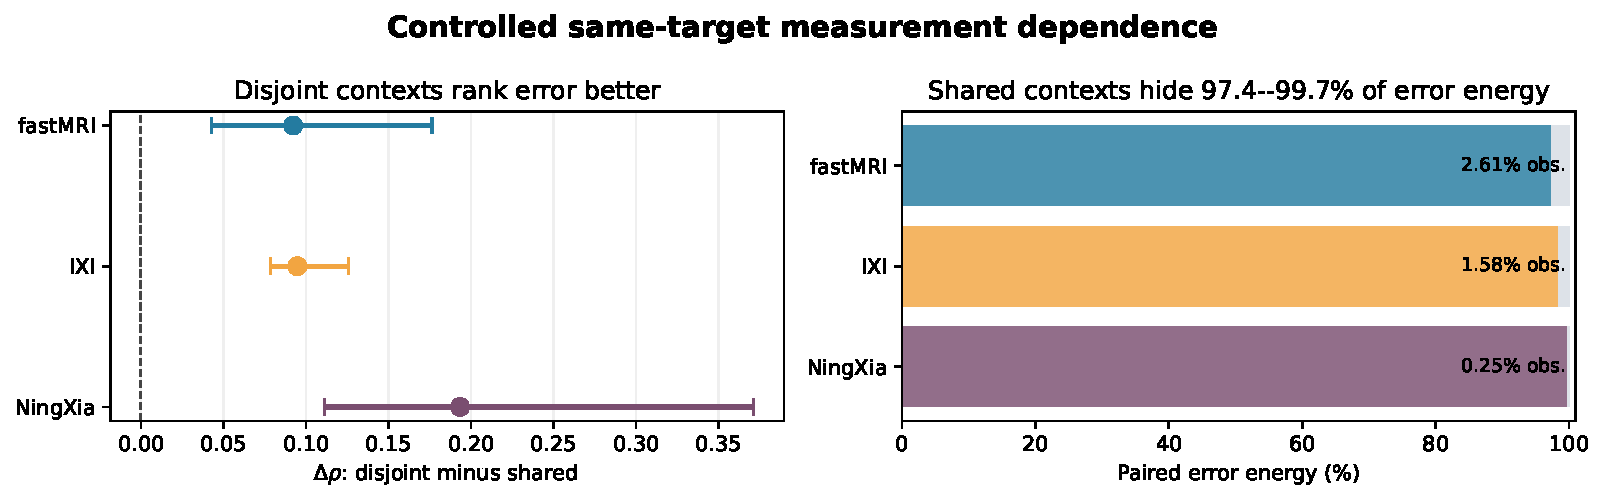
\includegraphics[width=.98\textwidth]{fig2_controlled_intervention.pdf}
\caption{Same-target controlled intervention. Left: error-ranking improvement of measurement-disjoint over clean dependence-preserving contexts, with clustered 95\% intervals. Right: shared (colored) and observable (gray) paired-error energy under clean sharing. NingXia uncertainty is patient-clustered over eight patients.}
\label{fig:control}
\end{figure*}

\subsection{Influence refines and survives falsification of count}
Raw count has the expected overall relationship with error geometry, but the exact compact ladder is not monotone. Across all cohorts, overlap-count trends are $+.9$ for error cosine/shared fraction and $-.9$ to $-1.0$ for observable fraction/disagreement; nevertheless, the zero-to-one transition reverses. The early claim that every added common anchor must reduce observability is therefore rejected.

Analytical influence resolves this exception. Common coefficient mass correlates with error alignment at .815, .789, and .855 on fastMRI, IXI, and NingXia, versus .503, .466, and .630 for count. Across alignment, shared fraction, observable fraction, and disagreement, every clustered interval for the absolute-correlation advantage of influence over count is above zero (.189--.283).

The nonlinear result is consistent across two architectures and three broad context grids (Fig.~\ref{fig:influence}). For error alignment, neural influence/count correlations are .838/.799 and .851/.796 on fastMRI, .797/.714 and .787/.712 on IXI, and .786/.743 and .772/.735 on NingXia for HAT/SwinIR. Across the 18 primary alignment/shared/observable endpoints, advantages range from .036 to .089 and every clustered interval excludes zero. Geometry- and examination-adjusted residual associations remain $|\rho|=.185$--.395.

\begin{figure*}[t]
\centering
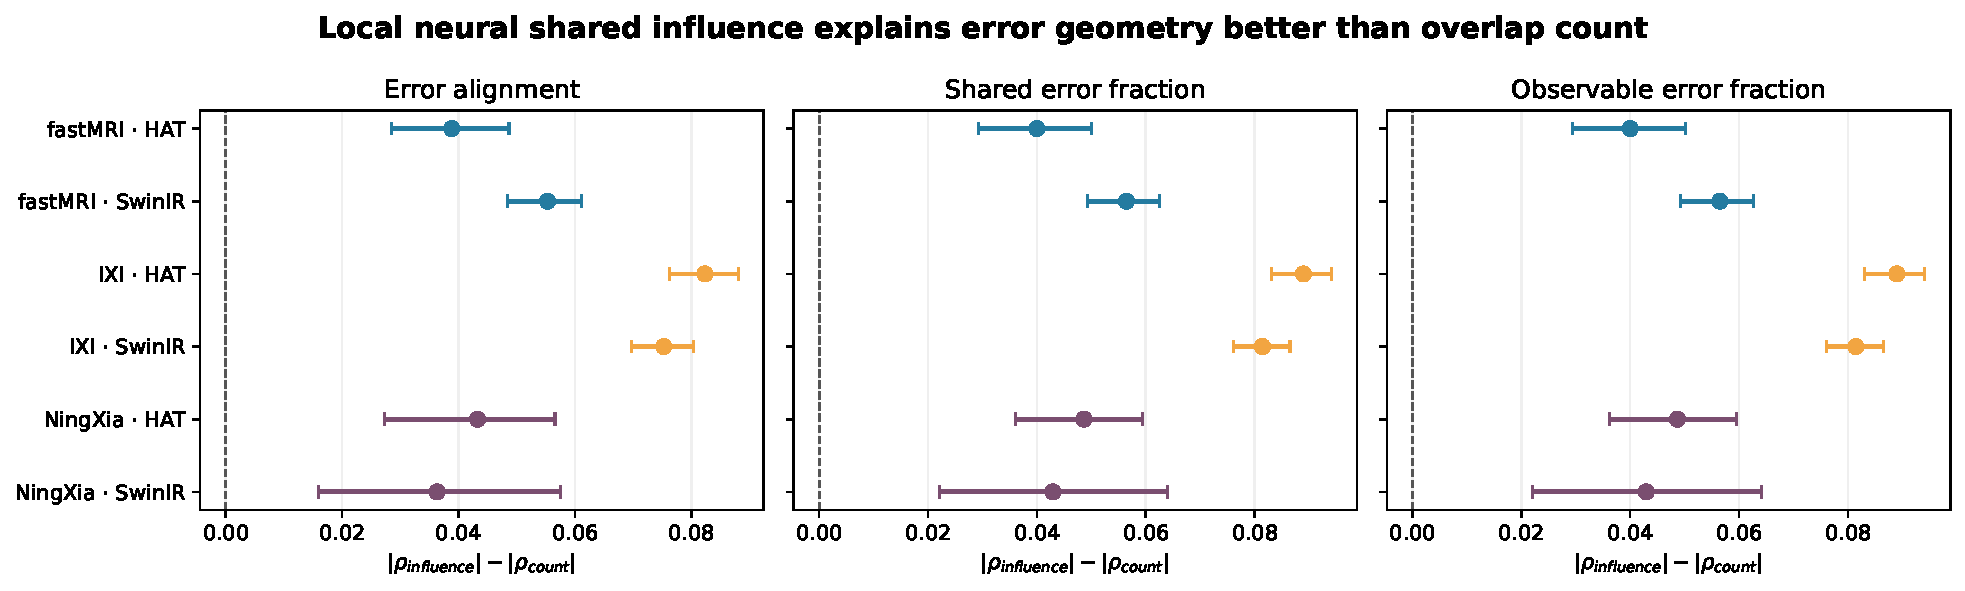
\includegraphics[width=.98\textwidth]{fig3_shared_influence.pdf}
\caption{Neural shared influence improves absolute association over raw anchor-overlap count for error alignment, shared error fraction, and observable error fraction in all six cohort--architecture strata. Points show $|\rho_{\rm influence}|-|\rho_{\rm count}|$ with examination/patient-clustered 95\% intervals.}
\label{fig:influence}
\end{figure*}

The exact-one-overlap subset is the decisive beyond-count boundary. After controlling span, asymmetry, and examination, neural influence retains the expected association for every endpoint/model on fastMRI and IXI ($|\rho|=.135$--.587; intervals exclude zero). NingXia does not replicate it: error-alignment partial $\rho$ is .014 for HAT and $-.039$ for SwinIR, all endpoint intervals cross zero, and some directions reverse. Thus the larger fastMRI/IXI cohorts support continuous influence beyond count; the eight-patient cohort supports only the broad descriptor and limits universal wording.

\begin{table*}[t]
\centering
\caption{Broad-grid and fixed-one-overlap neural evidence. Broad columns compare error-alignment correlation for count and neural influence; fixed columns give geometry/examination-adjusted influence correlation and clustered intervals.}
\label{tab:neural}
\setlength{\tabcolsep}{4pt}
\begin{tabular}{llrrrr}
\toprule
Cohort & Model & Broad $\rho_{\rm count}$ & Broad $\rho_{\rm influence}$ & Advantage [95\% CI] & Fixed-one-overlap partial $\rho$ [95\% CI] \\
\midrule
fastMRI & HAT & .799 & .838 & .039 [.028,.049] & .169 [.053,.283] \\
 & SwinIR & .796 & .851 & .055 [.048,.061] & .350 [.212,.464] \\
IXI & HAT & .714 & .797 & .082 [.076,.088] & .346 [.259,.424] \\
 & SwinIR & .712 & .787 & .075 [.070,.080] & .258 [.181,.335] \\
NingXia & HAT & .743 & .786 & .043 [.027,.057] & .014 [$-.232$,.223] \\
 & SwinIR & .735 & .772 & .036 [.016,.057] & $-.039$ [$-.175$,.144] \\
\bottomrule
\end{tabular}
\end{table*}

\subsection{The local mechanism is stronger than a global ranking law}
The arrow-wise analysis supports the local chain in all six strata. Influence-to-error-alignment partial $\rho$ is .219--.410; alignment-to-normalized-disagreement is $-.933$ to $-.889$; influence-to-observable-fraction is $-.412$ to $-.211$. All 18 intervals exclude zero. The context-level consequence is weaker: greater alignment predicts poorer disagreement--error ranking in all strata, but intervals exclude zero in only three of six. A local pair can have aligned errors because common anchors influence both predictions, while the global case-ranking effect also depends on anatomy, error magnitude, and the small set of contexts. This is evidence for a local mechanism, not causal mediation or a universal ranking theorem.

A prespecified stability audit strengthens this interpretation. All 42 amplitude, sign/field, and direction-count strata pass the rank-stability gate (minimum $\rho=.942$). Physical-plane rank stability is .779--.954 and only one of three plane-pair gates passes. The response statistic is numerically stable at a declared target/plane but not a plane-invariant global property.

\begin{table*}[t]
\centering
\caption{Mechanism-chain partial Spearman ranges across HAT/SwinIR. Every local-arrow interval excludes zero. The final column counts architecture strata with a context-ranking interval excluding zero.}
\label{tab:chain}
\setlength{\tabcolsep}{4pt}
\begin{tabular}{lrrrr}
\toprule
Cohort & Influence$\rightarrow$alignment & Alignment$\rightarrow$norm. disagreement & Influence$\rightarrow$observable & Alignment$\rightarrow$ranking \\
\midrule
fastMRI & .372--.410 & $-.933$--$-.926$ & $-.412$--$-.370$ & $-.333$--$-.143$ (0/2) \\
IXI & .321--.347 & $-.893$--$-.890$ & $-.342$--$-.298$ & $-.643$--$-.500$ (2/2) \\
NingXia & .219--.258 & $-.898$--$-.889$ & $-.231$--$-.211$ & $-.667$--$-.548$ (1/2) \\
\bottomrule
\end{tabular}
\end{table*}

\subsection{Practical consequence without superiority}
\begin{figure*}[t]
\centering
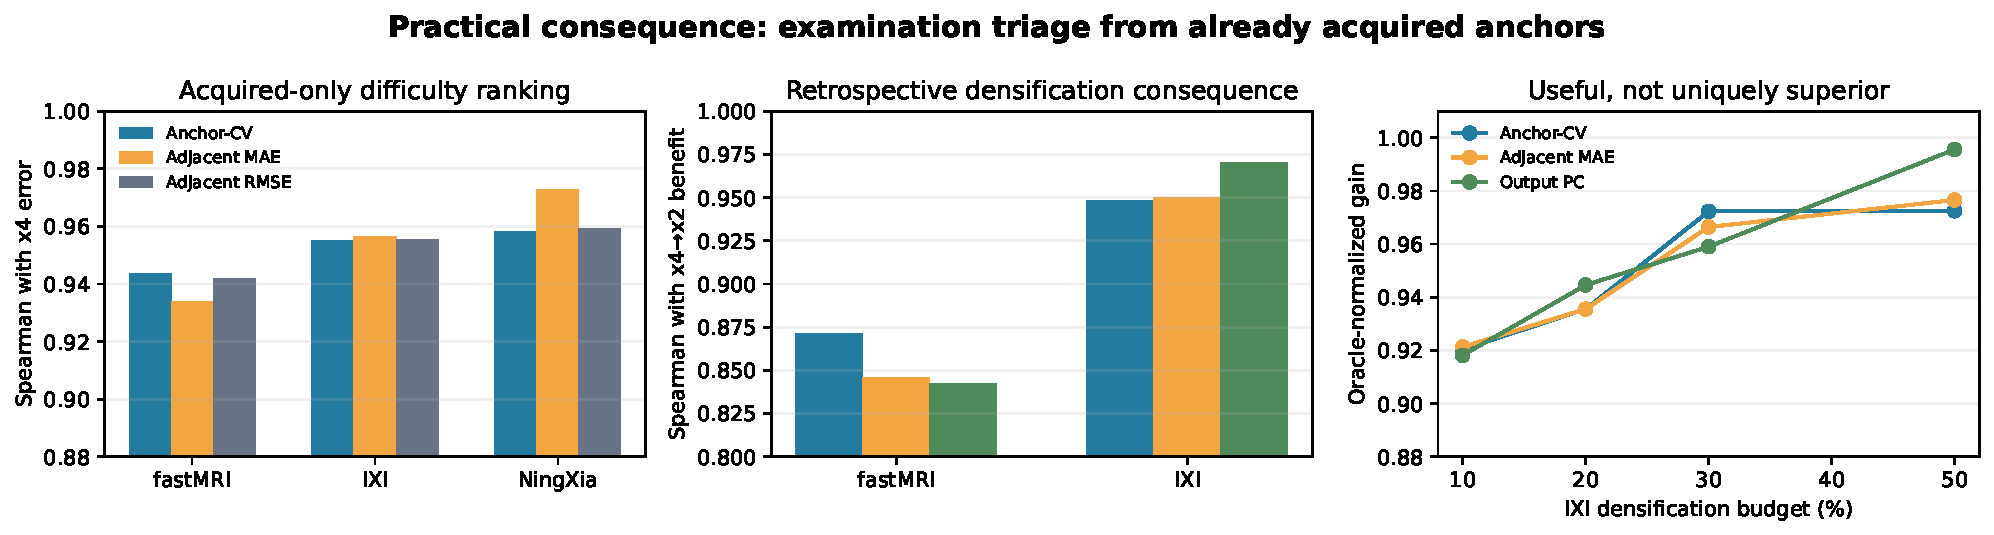
\includegraphics[width=.98\textwidth]{fig4_practical_consequence.pdf}
\caption{Practical consequence. Anchor-CV uses acquired anchors only and strongly ranks examination difficulty (left) and retrospective $\times4\!\rightarrow\!\times2$ benefit (middle). The IXI allocation curves (right) show large gain above random but no universal winner. Output PC requires existing reconstruction outputs; Anchor-CV requires none.}
\label{fig:consequence}
\end{figure*}

Figure~\ref{fig:consequence} evaluates acquired-anchor cross-validation as a consequence, not the central novelty. Anchor-CV ranks $\times4$ examination error with $\rho=.943/.955/.958$ on fastMRI/IXI/NingXia. Adjacent MAE gives .934/.956/.973 and adjacent RMSE .942/.956/.959; paired differences are not consistently significant. Conditional association beyond adjacent MAE, scale, and spacing is .333/$-.059$/$-.100$. Anchor-CV is therefore an interpretable acquired-only difficulty signal, not unique information.

The retrospective densification endpoint remains practically meaningful. Anchor-CV correlates with $\times4\!\rightarrow\!\times2$ benefit at .871 on fastMRI and .948 on IXI. On IXI its oracle-normalized gains are .920/.936/.972/.973 at the four frozen budgets. Adjacent MAE and output PC are comparable, and output PC reaches .970 benefit correlation and .996 gain at the 50\% IXI budget. The practical claim is availability and low cost: Anchor-CV requires already acquired anchors, zero dense targets at scoring, zero additional neural calls, and 0.42--3.97 ms CPU in the measured cases. It does not dominate every score.

\begin{table*}[t]
\centering
\caption{Practical consequence and strong baselines. Benefit is the retrospective $\times4\!\rightarrow\!\times2$ error reduction. Dashes indicate that NingXia is excluded from the frozen two-cohort consequence rule.}
\label{tab:practical}
\setlength{\tabcolsep}{4pt}
\begin{tabular}{lrrrr}
\toprule
Cohort & Anchor-CV $\rho$ vs. x4 error & Adjacent MAE $\rho$ & Anchor-CV $\rho$ vs. benefit & Best competing benefit $\rho$ \\
\midrule
fastMRI & .943 & .934 & .871 & .846 adjacent MAE / .843 PC \\
IXI & .955 & .956 & .948 & .970 PC \\
NingXia & .958 & .973 & --- & --- \\
\bottomrule
\end{tabular}
\end{table*}

\FloatBarrier

\raggedbottom
\section{Discussion}
The reviewer-memory message is simple: \emph{disagreement is only as informative as the independence of the information generating the compared predictions}. MRI interpolation makes this testable because target position and physical anchor identity are known. When contexts depend strongly on the same measurements, their local responses and target errors align, causing disagreement to understate error. Measurement-disjoint contexts expose a larger error component.

The progression from overlap count to influence is scientifically important. Count is attractive because it is exact and acquisition-only, but the zero-to-one reversal falsifies a strict dose law. Unequal coefficient mass explains analytical configurations, and paired neural finite responses transfer the idea to nonlinear interpolators. Plane dependence is not a failed invariance theorem because the final claim is local: influence belongs to a target--context--input configuration. It would contradict a claim of one intrinsic global model coefficient; we make no such claim.

The result also clarifies what is and is not actionable. Anchor-CV offers an inexpensive acquired-only examination signal and tracks retrospective densification value across fastMRI and IXI. Yet adjacent differences carry essentially the same rank information, output PC can be stronger when outputs already exist, and neither score localizes the worst physical plane. The mechanism therefore informs reliability-context design and examination triage without implying calibrated uncertainty, autonomous reacquisition, or a universally superior scalar.

Several limitations are material. NingXia contains 22 series but only eight independent patients; its fixed-count result is null/mixed. HAT and SwinIR are related 2.5-D interpolators, and all evaluated data are MRI T2. The neural context grid varies span/asymmetry, although partial controls and the fixed-count subset address this. Finite differences approximate local response under the chosen input fields and cannot identify a global Jacobian. The final context-ranking arrow is underpowered with eight configurations. The $\times2$ consequence is retrospective and cross-estimator on IXI; scanner time, motion, and clinical cost are absent. No result establishes diagnostic safety.

These boundaries also explain why several exploratory Plan-7 ideas are not paper contributions. Minimum-influence context selection, multi-anchor jackknife dispersion, and covariance residualization failed locked confirmation/transfer gates. Their failure prevents prescriptive claims but does not contradict the observed local relationship among measurement influence, error alignment, and cancellation. Complete exclusions and contradictions are audited in the supplement.

\paragraph{Evidence hierarchy.}
We treat fastMRI and IXI as the primary mechanism evidence because they provide 24 and 115 independent examinations. NingXia changes anatomy and site but contains eight patient clusters; it exposes heterogeneity rather than contributing artificial pooled precision. The same hierarchy is applied to favorable and unfavorable results: its broad influence direction is reported, and so is its exact fixed-count failure. This prevents both an underpowered nonreplication from erasing the primary effect and selective omission from overstating universality.

The broader relevance is a hypothesis rather than an empirical result. Any reliability system comparing predictions generated from shared measurements, features, priors, or training lineage may exhibit the same blind spot. Extending the physical intervention to other inverse problems is a useful next step; this paper's evidence remains scoped to MRI slice interpolation.

\begin{table*}[t]
\centering
\caption{Interpretation boundary. The right column lists the stronger inference that the submitted evidence does not support.}
\label{tab:boundary}
\setlength{\tabcolsep}{6pt}
\begin{tabular}{p{.46\textwidth}p{.46\textwidth}}
\toprule
Supported within the evaluated setting & Not supported \\
\midrule
Shared local measurement influence is associated with aligned error and reduced disagreement observability. & One plane-invariant global influence coefficient or causal mediation theorem. \\
Measurement-disjoint contexts expose more paired error than clean dependence-preserving controls. & A universal monotone law in raw anchor count or a guarantee for every context/dataset. \\
Anchor-CV ranks examination difficulty and retrospective densification value with no dense target at scoring. & A uniquely informative, calibrated, pixel-local, or universally superior uncertainty estimator. \\
The physical intervention motivates reliability design beyond one architecture. & Prospective scanner control, diagnostic safety, or empirical generalization outside MRI slice interpolation. \\
\bottomrule
\end{tabular}
\end{table*}

\FloatBarrier

\subsection{Operational reading and falsifiable predictions}
The mechanism changes how disagreement should be interpreted, not merely how it should be rescaled. A low disagreement value is reassuring only when the compared predictions draw on sufficiently independent influential information. In the evaluated interpolation setting, physical anchor identity supplies an auditable dependence label before reconstruction. Consequently, a reliability report should state both disagreement and the dependence of the contexts that produced it. Clean shared-anchor pairs are useful consistency controls; measurement-disjoint pairs are more diagnostic of error that shared inputs can conceal. These roles are complementary rather than interchangeable.

The result also yields tests that can fail. Holding target, anatomy, and model fixed, increasing \emph{shared influence} should increase error alignment and decrease the error component visible to prediction differences. Manipulating raw overlap without changing effective influence need not do so, as the observed zero-to-one reversal demonstrates. Likewise, changing plane or perturbation field may change the influence ordering; a claim of an intrinsic model-wide coefficient would therefore be falsified by the measured plane dependence. Future prospective studies can test whether deliberately diversified contexts improve error detection, but that intervention is not claimed here.

For deployment research, the immediate unit is the examination rather than a calibrated pixel. Anchor-CV can rank cases before dense targets exist, while adjacent-anchor differences provide a deliberately strong acquisition-only comparator and output PC is available after neural outputs are computed. The appropriate score depends on what is already available and on the downstream action. None of these retrospective rankings alone licenses reacquisition or diagnosis. A prospective decision rule would require an explicit cost function, scanner-time accounting, calibration on the intended population, and a safety study.

Finally, the negative results constrain follow-up work. New context-selection or covariance-correction methods should first pass the fixed-count test and transfer across both primary cohorts; success on pooled broad grids is insufficient. They should also report patient-clustered uncertainty and treat small external cohorts as heterogeneity probes rather than as a source of spurious precision. These requirements turn the present boundary findings into a concrete validation protocol without promoting the failed Plan-7 variants into contributions.

\section{Conclusion}
Deterministic MRI interpolators can agree while being jointly wrong because their errors share a component that prediction differences cannot observe. Controlled same-target interventions show that dependence-preserving contexts hide substantially more error than measurement-disjoint contexts across fastMRI, IXI, and NingXia. Integer overlap captures the trend but not the mechanism: analytical and local neural shared influence explain error alignment and observability more precisely. Acquired-anchor cross-validation supplies a lightweight examination-level consequence without being universally best. The strongest supported claim is narrow but consequential: reliability from disagreement depends on the independence of the influential information behind the predictions.

\clearpage
{\small
\bibliographystyle{ieeenat_fullname}
\bibliography{references}
}
\end{document}
